\chapter{Ajuste de \acrlongplsp{fcs} basado en descenso del gradiente}
\label{ch:fuzzy-controller-adjustment}

Como vimos en la sección~\ref{ss:fcs} del capítulo~\nameref{ch:sota-ci}, un \ac{fcs} se compone de cuatro bloques diferenciados: la fuzzificación, el bloque de reglas, la inferencia y la defuzzificación. De éstos bloques, el proceso manual de ajuste se resume siempre\sidenote{
	Por supuesto implica más ajustes como la elección de las funciones de fuzzificación, las $t$-normas y $t$-conormas, de la función de defuzzificación, pero estas operaciones no tienen tanto impacto en el desempeño del controlador como las particiones difusas y las reglas.
} en dos pasos:

\begin{enumerate}
	\item Elección de las particiones difusas de las variables lingüísticas.
	\item Definición de las reglas difusas.
\end{enumerate}

Las soluciones de ajuste que existen en la literatura suelen funcionar ajustando automáticamente uno de los dos puntos manteniendo constante el otro (e.g. ajustar las particiones manteniendo fijas las reglas). Nosotros representaremos el controlador como un grafo computacional de manera que sus gradientes sean sencillos de ajustar\sidenote{
	Como veremos más adelante, el tiempo de ajuste con esta representación es muy rápido, lo que abre la posibilidad de desarrollar un algoritmo que incluya este para el ajuste de los metaparámetros del controlador, como por ejemplo los tamaños de las particiones.
}.

Se han tomado una serie de decisiones de diseño para facilitar el desarrollo del controlador, aunque son fácilmente modificables. Éstas son:

\begin{itemize}
	\item Para cada partición difusa se limitarán las funciones de pertenencia a: una línea descendente para caracterizar al primer conjunto difuso, una línea ascendente para caracterizar el último y trapezoides para caracterizar al resto.
	\item Las $t$-norma y $t$-conorma serán el máximo y el mínimo respectivamente. La $t$-norma se usará como operador asociado al \texttt{AND} lógico y a la operación de implicación, mientras que la $t$-conorma se usará como operador asociado al \texttt{OR} lógico y a la acumulación.
	\item El controlador será de tipo \textit{Takagi-Sugeno} de orden $0$, y por tanto se representarán las funciones de salida como conjuntos difusos de tipo singletón. La función de defuzzificación será la la operación CoGS\sidenote{
		La operación CoGS (\textit{Center of Gravity for Singletons}) se define como:
		\begin{equation}
			CoGS = \sum_{i=1}^n w_i \cdot o_i
			\label{eq:cogs}
		\end{equation}
		Es decir, la suma ponderada de los valores de salida.
	}.
	\item El tamaño de las particiones difusas no variará dinámicamente a lo largo del entrenamiento, siendo este un meta-parámetro de configuración del controlador.
	\item El controlador tendrá una única variable de salida.
\end{itemize}

\section{El \acrlongsp{fcs} como grafo computacional}

Sea $\mathcal{V} = {V_1, V_2, \ldots, V_n}$ el conjunto ordenado de variables lingüísticas de nuestro controlador, y sea $O$ la variable lingüística de salida. Cada una de estas variables tendrá un número prefijado de conjuntos $\mathcal{N} = {N_{V_1}, N_{V_2}, \ldots, N_{V_n}}$ para las variables de entrada y $N_O$ para la variable de salida.

El controlador recibirá una matriz bidimensional de rango $(m, n)$ y devolverá un vector de rango $(m)$, siendo $m$ el número de ejemplos que queremos calcular a la vez.

Representaremos el \ac{fcs} como grafo computacional. De esta manera, podremos (i) aplicar la función de manera más eficiente y (ii) calcular fácilmente los gradientes de las funciones parciales para aplicar la técnica del descenso del gradiente propagando el error de la salida.

El proceso de desarrollo será el siguiente: primero, construiremos cada uno de los bloques fundamentales del \ac{fcs} como un grafos computacionales; después construiremos el controlador conectando entre sí estos grafos.

\subsection{Bloque de fuzzificación}

El grafo computacional asociado a este bloque tomará una matrix bidimensional de rango $(m, n)$ (la matriz de entrada) que contendrá para cada ejemplo una lista de los valores que toma cada una de las variables de entrada. La salida de este grafo será una matriz bidimensional de rango $(m, \sum_{i=1}^n N_i)$, donde se almacenarán los grados de pertenencia de esos valores acada conjunto difuso de la variable que les corresponda (Figura~\ref{fig:input-to-fuzzy-input}).

\begin{figure*}[t]
	\centering
	\begin{equation*}
		\left(\begin{array}{>{\columncolor{red!20}}c>{\columncolor{blue!20}}cc}
		x^1_{V_1} & x^1_{V_2} & \ldots \\
		x^2_{V_1} & x^2_{V_2} & \ldots \\
		x^3_{V_1} & x^3_{V_2} & \ldots \\
		x^4_{V_1} & x^4_{V_2} & \ldots \\
		\end{array}\right)
		\quad \rightarrow \quad 
		\left(\begin{array}{>{\columncolor{red!20}}c>{\columncolor{red!20}}c>{\columncolor{blue!20}}c>{\columncolor{blue!20}}cc}
		\mu^1_{V_1}(x^1_{V_1}) & \mu^2_{V_1}(x^1_{V_1}) & \mu^1_{V_2}(x^1_{V_2}) & \mu^2_{V_2}(x^1_{V_2}) & \ldots \\
		\mu^1_{V_1}(x^2_{V_1}) & \mu^2_{V_1}(x^2_{V_1}) & \mu^1_{V_2}(x^2_{V_2}) & \mu^2_{V_2}(x^2_{V_2}) & \ldots \\
		\mu^1_{V_1}(x^3_{V_1}) & \mu^2_{V_1}(x^3_{V_1}) & \mu^1_{V_2}(x^3_{V_2}) & \mu^2_{V_2}(x^3_{V_2}) & \ldots \\
		\mu^1_{V_1}(x^4_{V_1}) & \mu^2_{V_1}(x^4_{V_1}) & \mu^1_{V_2}(x^4_{V_2}) & \mu^2_{V_2}(x^4_{V_2}) & \ldots \\
		\end{array}\right)
	\end{equation*}
	\caption[Ejemplo de operación en el bloque de fuzzificación]{El bloque de fuzzificación transformará los valores de sus respectivos dominios al dominio de pertenencia a cada conjunto difuso. La matriz generada tendrá tantas columnas como conjuntos difusos posea cada variable.}
	\label{fig:input-to-fuzzy-input}
\end{figure*}

Para ello, se le aplicará a cada columna de la matriz de entrada tantas operaciones (funciones de pertenencia) como conjuntos difusos posea. Concretamente se aplicarán operaciones de línea descendente, trapezoidal y ascendente.

Las líneas \textbf{ascendente} y \textbf{descendente} tienen una forma parecida. El grafo asociado a la fórmula de la línea descendente se muestra en la figura~\ref{fig:slope-asc-grap}, que es la que se correspondería con el último conjunto de una partición difusa. Como se puede ver, las variables ajustables son $a$ y $\delta a$. Estas definen el intervalo $(a, a + \delta b) \in \mathbb{R}$ donde los valores $f(X)$ ascienden de $0$ a $1$ (o descienden de $1$ a $0$ en el caso de la recta ascendente).

\begin{figure}
	\centering
	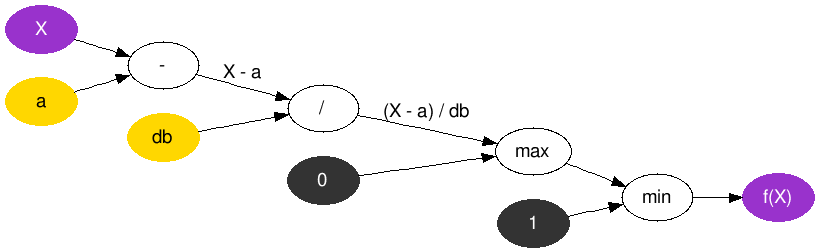
\includegraphics{slope-asc-graph}
	\caption[Grafo computacional de la función de pertenencia para la línea ascendente]{Ilustración del grafo computacional para la función de pertenencia línea ascendente. La fórmula que describe es $\mu(x) = \min(\max(\frac{x - a}{\delta b}, 0), 1)$, quedando acotada $\mu(x)$ en el intervalo $[0, 1] \in \mathbb{R}$. El grafo computacional para la línea descendente es similar y se corresponde con la fórmula $\mu(x) = \min(\max(\frac{a - x}{\delta b + 1}, 0), 1)$.}
	\label{fig:slope-asc-grap}
\end{figure}

El \textbf{trapecio} se define a partir de los parámetros $(a, \delta b, \delta c, \delta d) \in \mathbb{R}$, que definen los intervalos $I_1 = (a, a + \delta b)$, $I_1 = (a + \delta b, a + \delta b + \delta c)$ y $I_3 = (a + \delta b + \delta c, a + \delta b + \delta c + \delta d)$. $I_1$ es el intervalo donde la función de pertenencia aumenta su valor de $0$ a $1$, $I_2$ el intervalo superior del trapecio donde la función vale $1$ e $I_3$ donde la función comienza a descender su valor de $1$ a $0$. El grafo asociado a esta función se ilustra en la figura~\ref{fig:trap-graph}

\begin{figure}
	\centering
	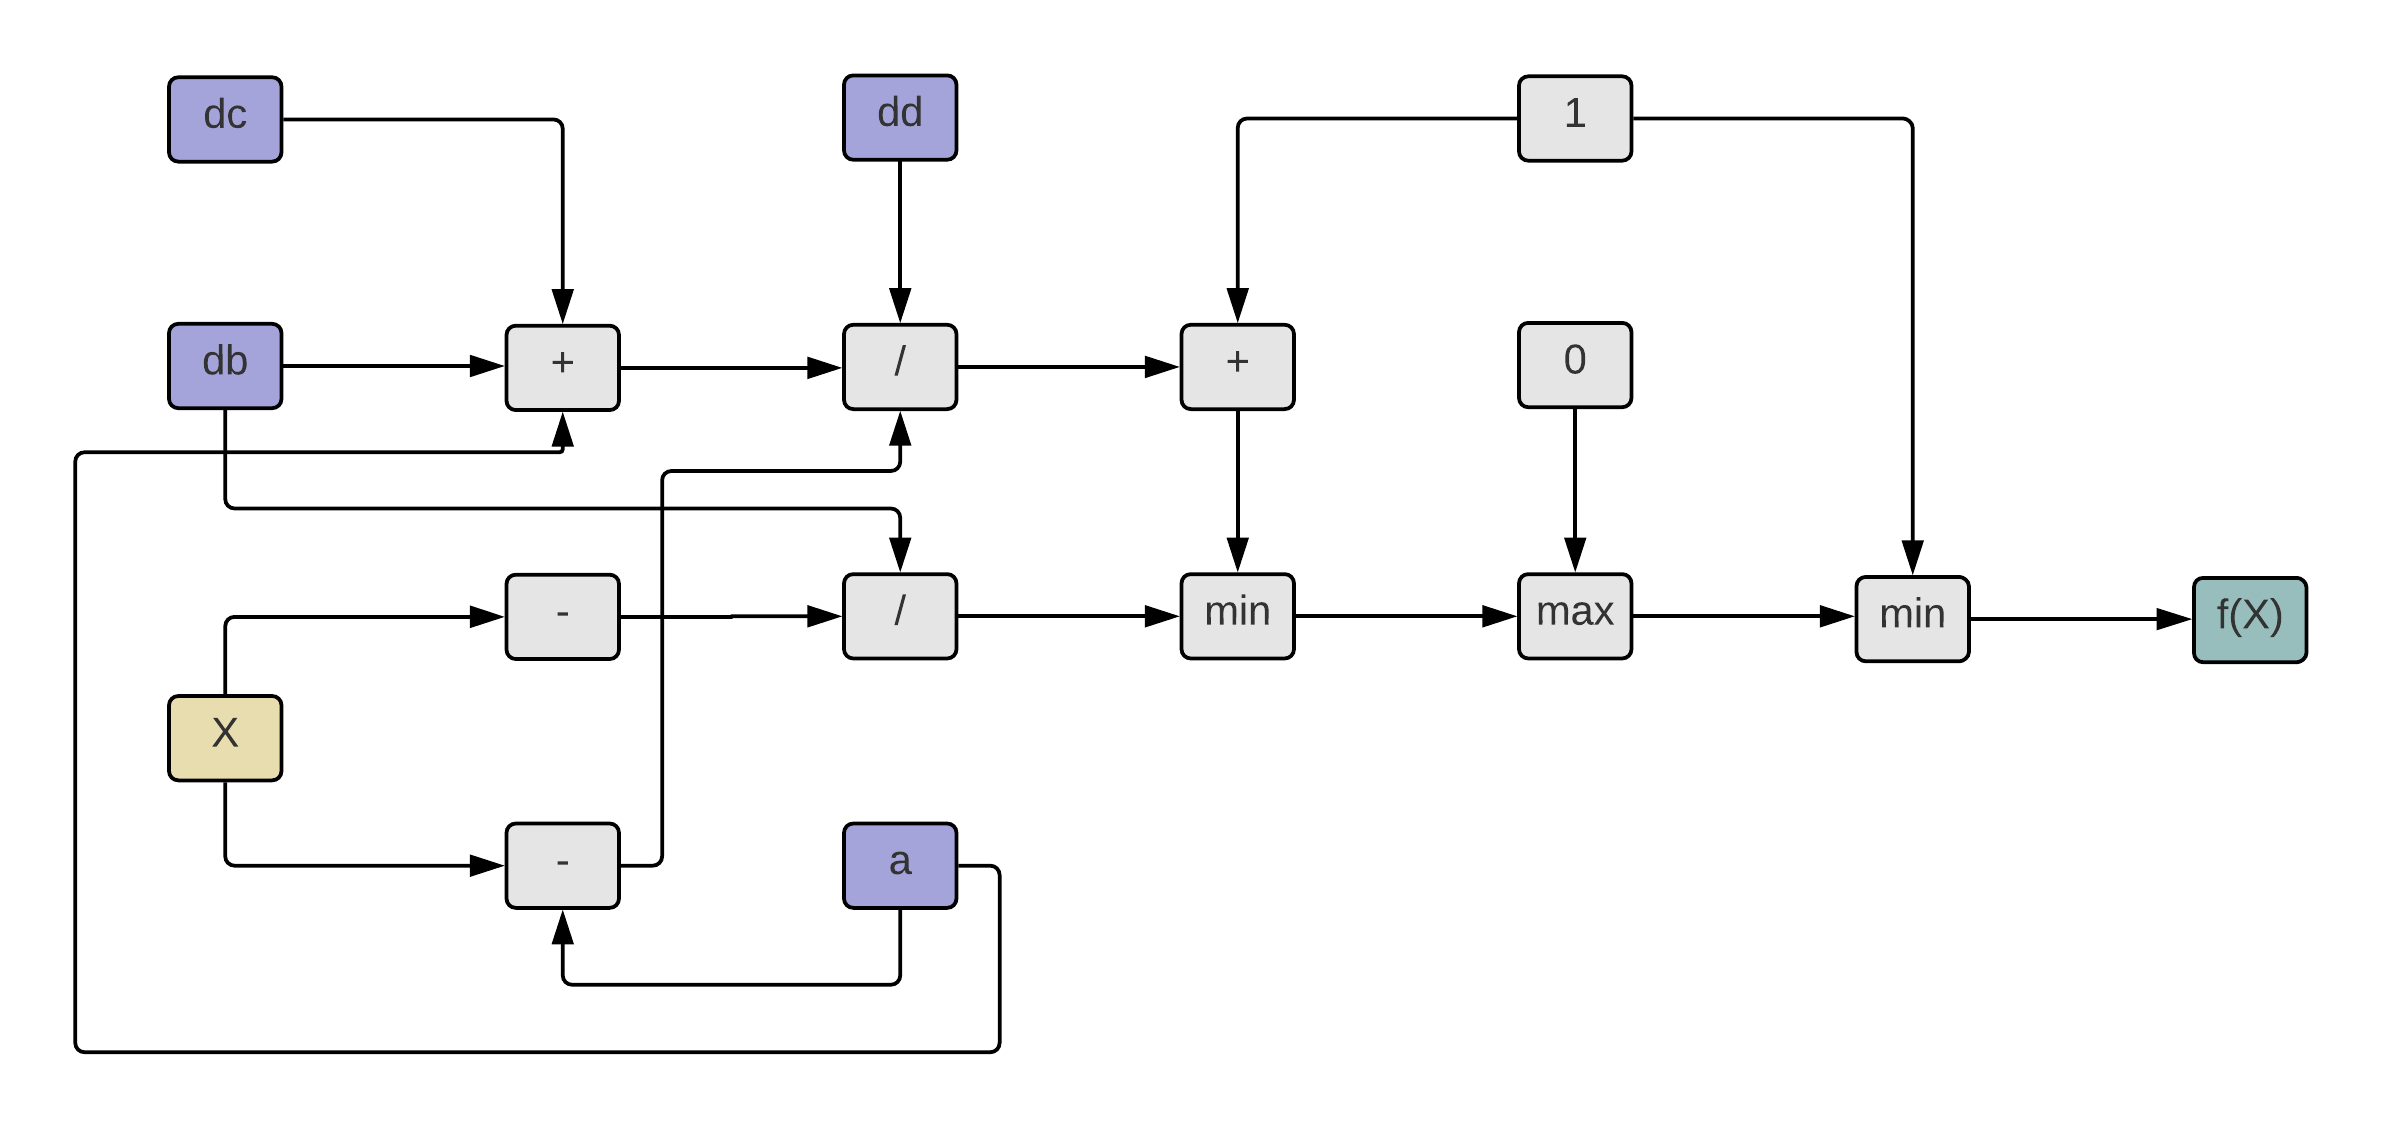
\includegraphics{trap-graph}
	\caption[Grafo computacional de la función de pertenencia para el trapecio]{Ilustración del grafo computacional para la función de pertenencia trapezoidal. La fórmula que describe es $\mu(x) = \min(\max(\min(\mu_{L_{asc}}, \mu_{L_{desc}}), 0), 1)$, esto es, una línea ascendente y otra descendente, estando ambas acotadas en el intervalo $[0, 1] \in \mathbb{R}$.}
	\label{fig:trap-graph}
\end{figure}

Sabiendo los grafos computacionales de cada una de las funciones de pertenencia, ya podemos definir el grafo asociado a la partición difusa de una variable lingüística. Suponiendo que la variable $V_i$ está dividida en $N_{V_i}$ conjuntos difusos, la partición de ésta estará compuesta de:

\begin{itemize}
	\item Un primer conjunto definido como una pendiente descendente.
	\item $N_{V_i} - 2$ conjuntos definidos por una función de pertenencia de tipo trapezoidal.
	\item Un último conjunto definido como una pendiente ascendente.
\end{itemize}

Este grafo tiene que definir una serie de variables para que nuestro algoritmo de entrenamiento las ajuste correctamente. Estas variables están directamente relacionadas con los parámetros de las funciones de pertenencia descritas anteriormente. Hemos decidido por tanto establecer estas variables como los espacios existentes entre los puntos caracteríscos de las funciones. En la figura~\ref{fig:fuzzification-graph-vars} se puede observar de qué manera están relacionadas las variables de desplazamiento y los parámetros de las funciones de pertenencia.

Al estar definidas de esta manera, logramos (i) que la suma de todas las pertenencias en cada punto del eje $X$ es $1$ y (ii) que cada pequeña variación del gradiente de una de las variables tiene el potencial de provocar una variación en el resto de variables.

Por último, un controlador difuso define un número de variables de entrada. Nuestro grafo de fuzzificación estará definido de tal manera que para una matriz de entrada $m \times l$, siendo $m$ cada tupla de valores a inferir y $l$ cada una de las variables lingüísticas, generará una matriz de la forma $m \times \sum_{i=1}^l \left\vert{l_i}\right\vert$, siendo $\left\vert{S}\right\vert$ el número de conjuntos difusos que contiene la variable linguística $l_i$ (Figura~\ref{fuzzification-graph})

\begin{figure}
	\centering
	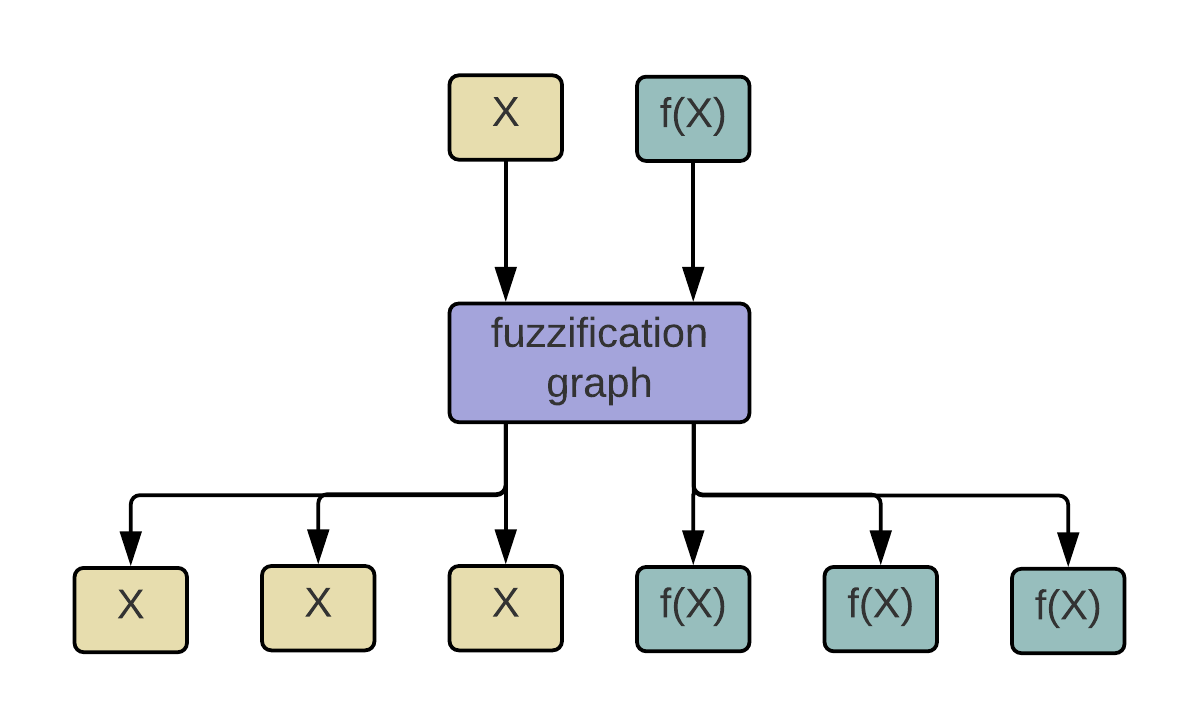
\includegraphics{fuzzification-graph}
	\caption[Ejemplo de operación de fuzzificación como grafo computacional]{Siendo el número de conjuntos difusos de las variables lingüísticas $X_1$ e $X_2$ $3$, el grafo de fuzzificación transformará los dos valores de entrada $x \in X_1$ e $y \in X_2$ en seis valores, los corerspondientes a los valores de pertenencia de $x$ e $y$ a cada uno de los conjuntos difusos de $X_1$ y $X_2$ respectivamente}
	\label{fig:fuzzification-graph}
\end{figure}

\subsection{Bloque de inferencia}

Este bloque tomará una matriz bidimensional de rango $(m, \sum_{i=1}^n N_i)$, es decir, la matriz de salida del bloque de fuzzificación, y generará una matriz bidimensional de rango $(m, N_O)$ que contendrá los valores difusos de salida (un valor difuso por cada conjunto difuso de salida). Para ello, hará uso de un bloque de reglas en las que basará su inferencia.

Este bloque de reglas es el que se tratará de ajustar. La representación será la de una matriz $(v_i + 1)$-dimensional, siendo $v_i = \sum_{i=1}^l \left\vert{l_i}\right\vert$ (el número total de entradas difusas que llegan al bloque). La dimensión adicional se corresponde a la variable lingüística de salida.

Dicho de otro modo, cada posible conjunto difuso de salida (es decir, para cada valor dentro del eje correspondiente a la salida) se corresponderá con una matriz $v_i$-dimensional resultado del producto cartesiano de las cariables de entradas. Esto es, cada una de las posibles combinaciones de reglas, a la que podemos asociar un valor. En la Figura~\ref{fig:inference-graph} se muestra un ejemplo con las variables obtenidas en el ejemplo de la Figura~\ref{fig:fuzzification-graph} tras aplicarles la $t$-norma.


\begin{figure*}[t]
	\centering
	\begin{equation*}
		\left(\begin{array}{c}
			\mu_1^A \ldots \\
			\mu_2^A \ldots \\
			\mu_3^A \ldots \\
		\end{array}\right)
		\quad \times \quad
		\left(\begin{array}{ c}
			\mu_1^B \ldots \\
			\mu_2^B \ldots \\
			\mu_3^B \ldots \\
		\end{array}\right)
		= \quad 
		\left(\begin{array}{c}
			\top(\mu_1^A, \mu_1^B) \\
			\top(\mu_1^A, \mu_2^B) \\
			\top(\mu_1^A, \mu_3^B) \\
			\top(\mu_2^A, \mu_1^B) \\
			\top(\mu_2^A, \mu_2^B) \\
			\top(\mu_2^A, \mu_3^B) \\
			\top(\mu_3^A, \mu_1^B) \\
			\top(\mu_3^A, \mu_2^B) \\
			\top(\mu_3^A, \mu_3^B) \\
		\end{array}\right)
	\end{equation*}
	\caption[Producto cartesiano de variables difusas de entrada]{El producto cartesiano de las variables difusas de entrada genera todas las posibles combinaciones entre los conjuntos difusos de las variables lingüísticas. Aplicándosele la $t$-norma a cada una de estas combinaciones tenemos todas las posibles reglas que se pueden definir en este \acrlong{fcs}.}
	\label{fig:inference-graph}
\end{figure*}

Al estar definida la $t$-conorma y la acumulación con el mismo operador (i.e. el máximo), una regla de tipo OR es equivalente a dos reglas de tipo AND, ya que la acumulación de sus resultados es equivalente. Por tanto, al aplicar la $t$-norma a estas combinaciones tenemos todas las posibles combinaciones de reglas. Pero hasta aquí no tenemos ningún ajuste.

Si aplicamos el producto de Hadamard a una matriz de pesos con la misma dimensión y acotamos sus valores a $[0, 1] \in \mathbb{N}$, tenemos una manera de ajustar qué reglas son las más relevantes y cuáles no. Esta representación tiene un problema: estos dos valores definen una función escalón donde el error no se propaga al ser su gradiente $0$. Sin embargo, si en lugar de un valor natural, el peso toma un valor real y le aplicamos una operación sigmoidal, el valor se mantendrá entre $(0, 1) \in \mathbb{R}$ con la ventaja de que el gradiente no se estanca, y en un proceso posterior se pueden descartar las reglas cuyos valores superen ciertos rangos establecidos.

A la salida de la inferencia, tras aplicar la acumulación, disponemos de tantos valores difusos como conjuntos difusos tiene la salida.

\subsection{Bloque de defuzzificación}

Este bloque tiene la particularidad de que no posee ninguna variable que ajustar. Se trata simplemente de una operación que toma una matriz bidimensional de rango $(m, N_O)$ con los valores difusos de salida y devuelve un vector de rango $(m)$ con los valores en el dominio de la variable lingüística de salida.

\section{Ejemplo de ajuste de un controlador difuso}

Para probar su funcionamiento, se realizará el ajuste de un controlador difuso a partir de un conjunto de entrenamiento con unos valores determinados. Estos valores se habrán obtenido a su vez de un \ac{fcs} de ejemplo para comprobar lo correcto de la implementación.

\begin{figure}
	\centering
	\subfloat[Variable \textit{Food}]{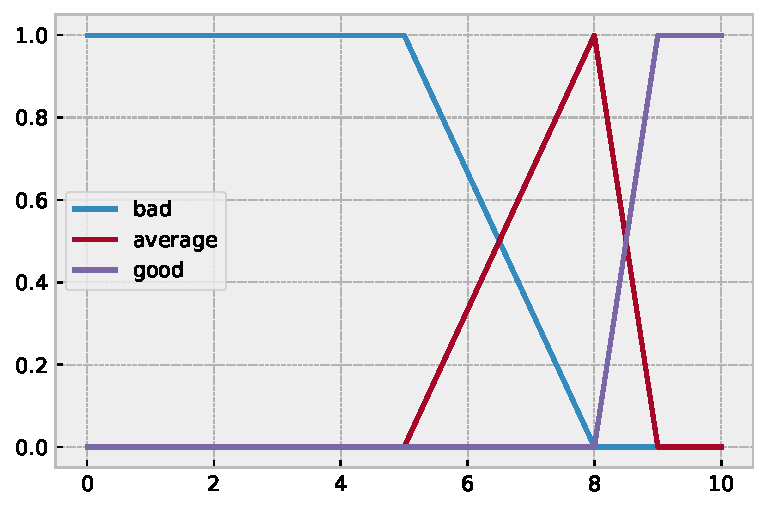
\includegraphics[width=.45\textwidth]{real-tip-controller-var-food}}\qquad
	\subfloat[Variable \textit{Service}]{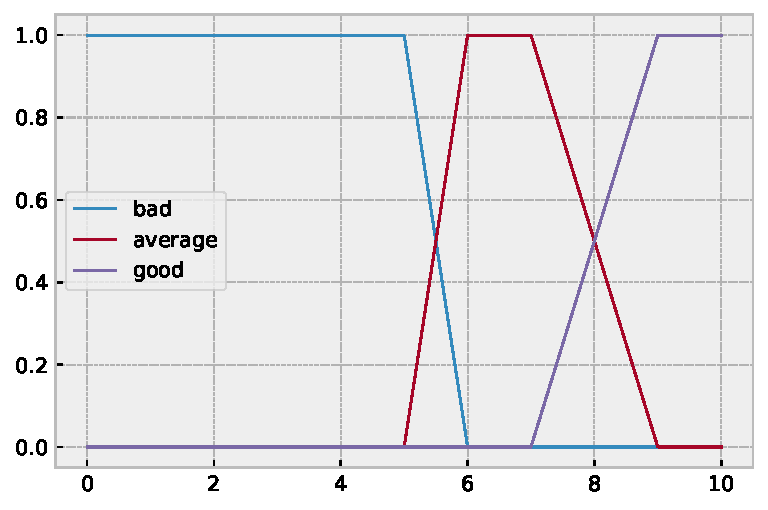
\includegraphics[width=.45\textwidth]{real-tip-controller-var-service}}
	\caption[Particiones difusas del controlador de ejemplo]{Particiones difusas del controlador de ejemplo. Estas particiones junto con las reglas definirán la superficie de la función que modela nuestro controlador de ejemplo.}
	\label{fig:real-tip-controller-vars}
\end{figure}


El ejemplo en concreto se trata del problema clásico de la asignación de propinas, donde la propina viene determinada en función de las variables calidad de la comida y calidad del servicio. Las particiones de las variables lingüísticas del controlador (denominadas \textit{food} y \textit{service}) se muestran en la Figura~\ref{fig:real-tip-controller-vars}. Las reglas que determinan su comportamiento son las siguientes:

\begin{align}
	\text{service IS good}                              &\rightarrow \text{tip IS high}\nonumber\\
	\text{food IS good}                                 &\rightarrow \text{tip IS high}\nonumber\\
	\text{service IS good} \land \text{food IS average} &\rightarrow \text{tip IS low}\nonumber\\
	\text{service IS average} \land \text{food IS good} &\rightarrow \text{tip IS high}\nonumber\\
	\text{service IS bad}                               &\rightarrow \text{tip IS low}\nonumber\\
	\text{food IS bad}                                  &\rightarrow \text{tip IS low}
\end{align}

El controlador es una función con dos variables que describen la superficie mostrada en la Figura~\ref{fig:real-tip-controller-surface}.

\begin{figure}
	\centering
	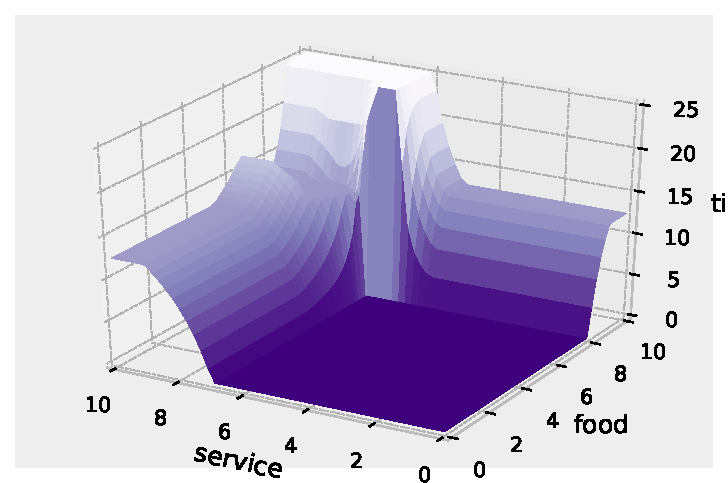
\includegraphics{real-tip-controller-surface}
	\caption[Superficie de la función que modela el \acrlongsp{fcs} de ejemplo]{Las reglas y las particiones definen esta función. De ella obtendremos un conjunto de puntos aleatorio para comprobar si nuestra representación de \acrlongsp{fcs} como grafo computacional es capaz de ajustarse a ésta con la técnica del descenso del gradiente.}
	\label{fig:real-tip-controller-surface}
\end{figure}

Recogeremos una muestra aleatoria uniforme de $2500$ de entre los $62500$ que conforman la representación de la superficie del controlador de ejemplo. Posteriormente se crea un controlador difuso y se itera el algoritmo de descenso del gradiente ADAM~\cite{kingma2014adam}.

El proceso de entrenamiento consistirá en la ejecución del algoritmo de propagación del error durante $2500$ epochs con una tasa de aprendizaje de $0.01$, la cual se ha considerado suficiente para el ejemplo en cuestión. La evolución del error durante este entrenamiento se puede ver en la Figura~\ref{fig:fcs-ajustment-rms-during-training}.

Durante el entrenamiento, las superficies evolucionan hacia una representación aproximada de lo que es el controlador original. En la figura~\ref{fig:adjusted-tip-controller-training} podemos observar cómo evoluciona la superficie que representa el controlador ajustado.

\begin{figure}
	\centering
	\subfloat[Inicio]{\includegraphics[width=.28\textwidth]{ajusted-tip-controller-at-start-training}}\qquad
	\subfloat[Epoch $250$]{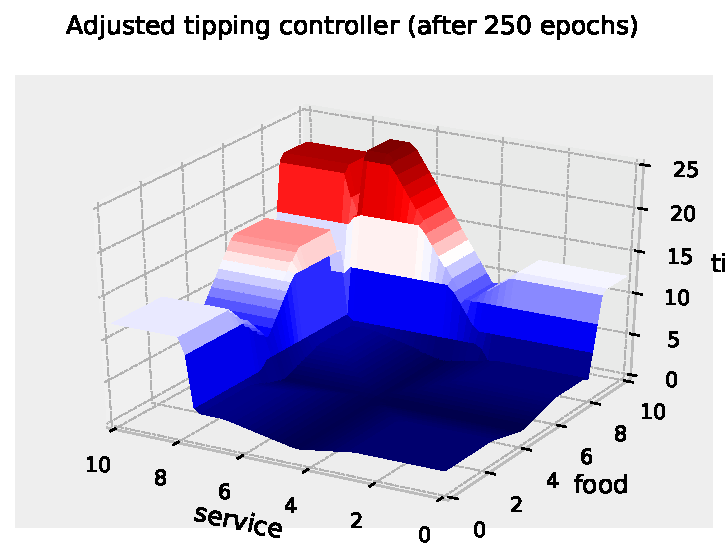
\includegraphics[width=.28\textwidth]{ajusted-tip-controller-at-half-training}}\qquad
	\subfloat[Epoch $1000$]{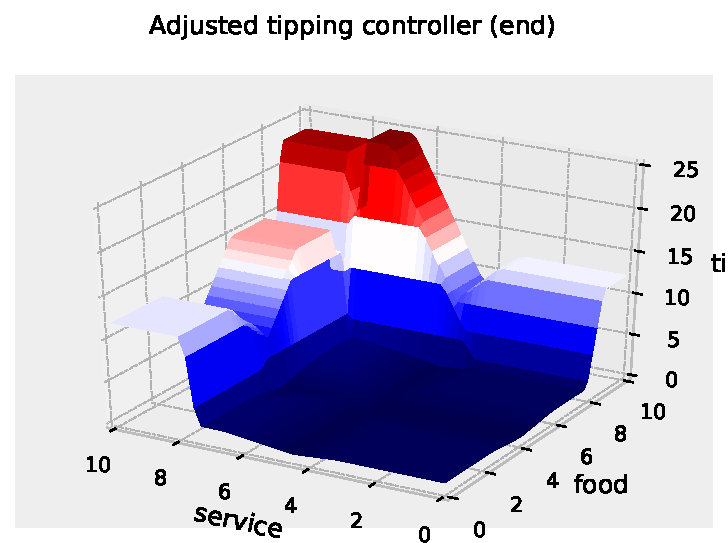
\includegraphics[width=.28\textwidth]{ajusted-tip-controller-at-end-training}}
	\caption[Evolución del \acrlongsp{fcs} de acuerdo al conjunto de datos extraido del ]{Particiones difusas del \acrlongsp{fcs} de ajustado. Estas figuras muestran la superficie del controlador ajustado (a) al comienzo del proceso de entrenamiento, (b) tras $250$ iteraciones sobre el conjunto de entrenamiento y (c) al final del proceso del entrenamiento.}
	\label{fig:adjusted-tip-controller-training}
\end{figure}

Este proceso demuestra que es posible obtener controladores difusos ajustados a un patrón de datos con un grado alto de precisión. La ventaja de este método radica en que es posible por tanto explicar mediante reglas el por qué de las predicciones que hace el modelo, a diferencia de otras técnicas como las \ac{ann}\sidenote{Aunque no se han extraído en este ejemplo, el proceso de extracción de particiones difusas y reglas se muestra en el capítulo~\nameref{ch:lane-change-model}.}.